This section outlines the \textbf{InternHub – Students \& Companies (S\&C)} platform's user interface, including a summary of the main pages that make up the system. Since changes to the design may be made throughout the testing phase, the design mockups displayed here focus more on the interface's usability and interaction dynamics than on its final visual aesthetics. Equivalent pages will be made for mobile devices, even if the desktop browser version is the main focus due to its suitability for thorough profile management and internship-related procedures. By adapting and scaling the interface to fit smaller screens, this guarantees a seamless user experience.

The design prototypes shown here serve as a fundamental depiction of the platform's user interface, as specified in the \textbf{RASD}. As the system develops, these designs are subject to optimization and improvement, taking into account input from user interactions and testing.

\section{Overview}
\label{sec:overview}%
\begin{figure}[H]
    \begin{center}
        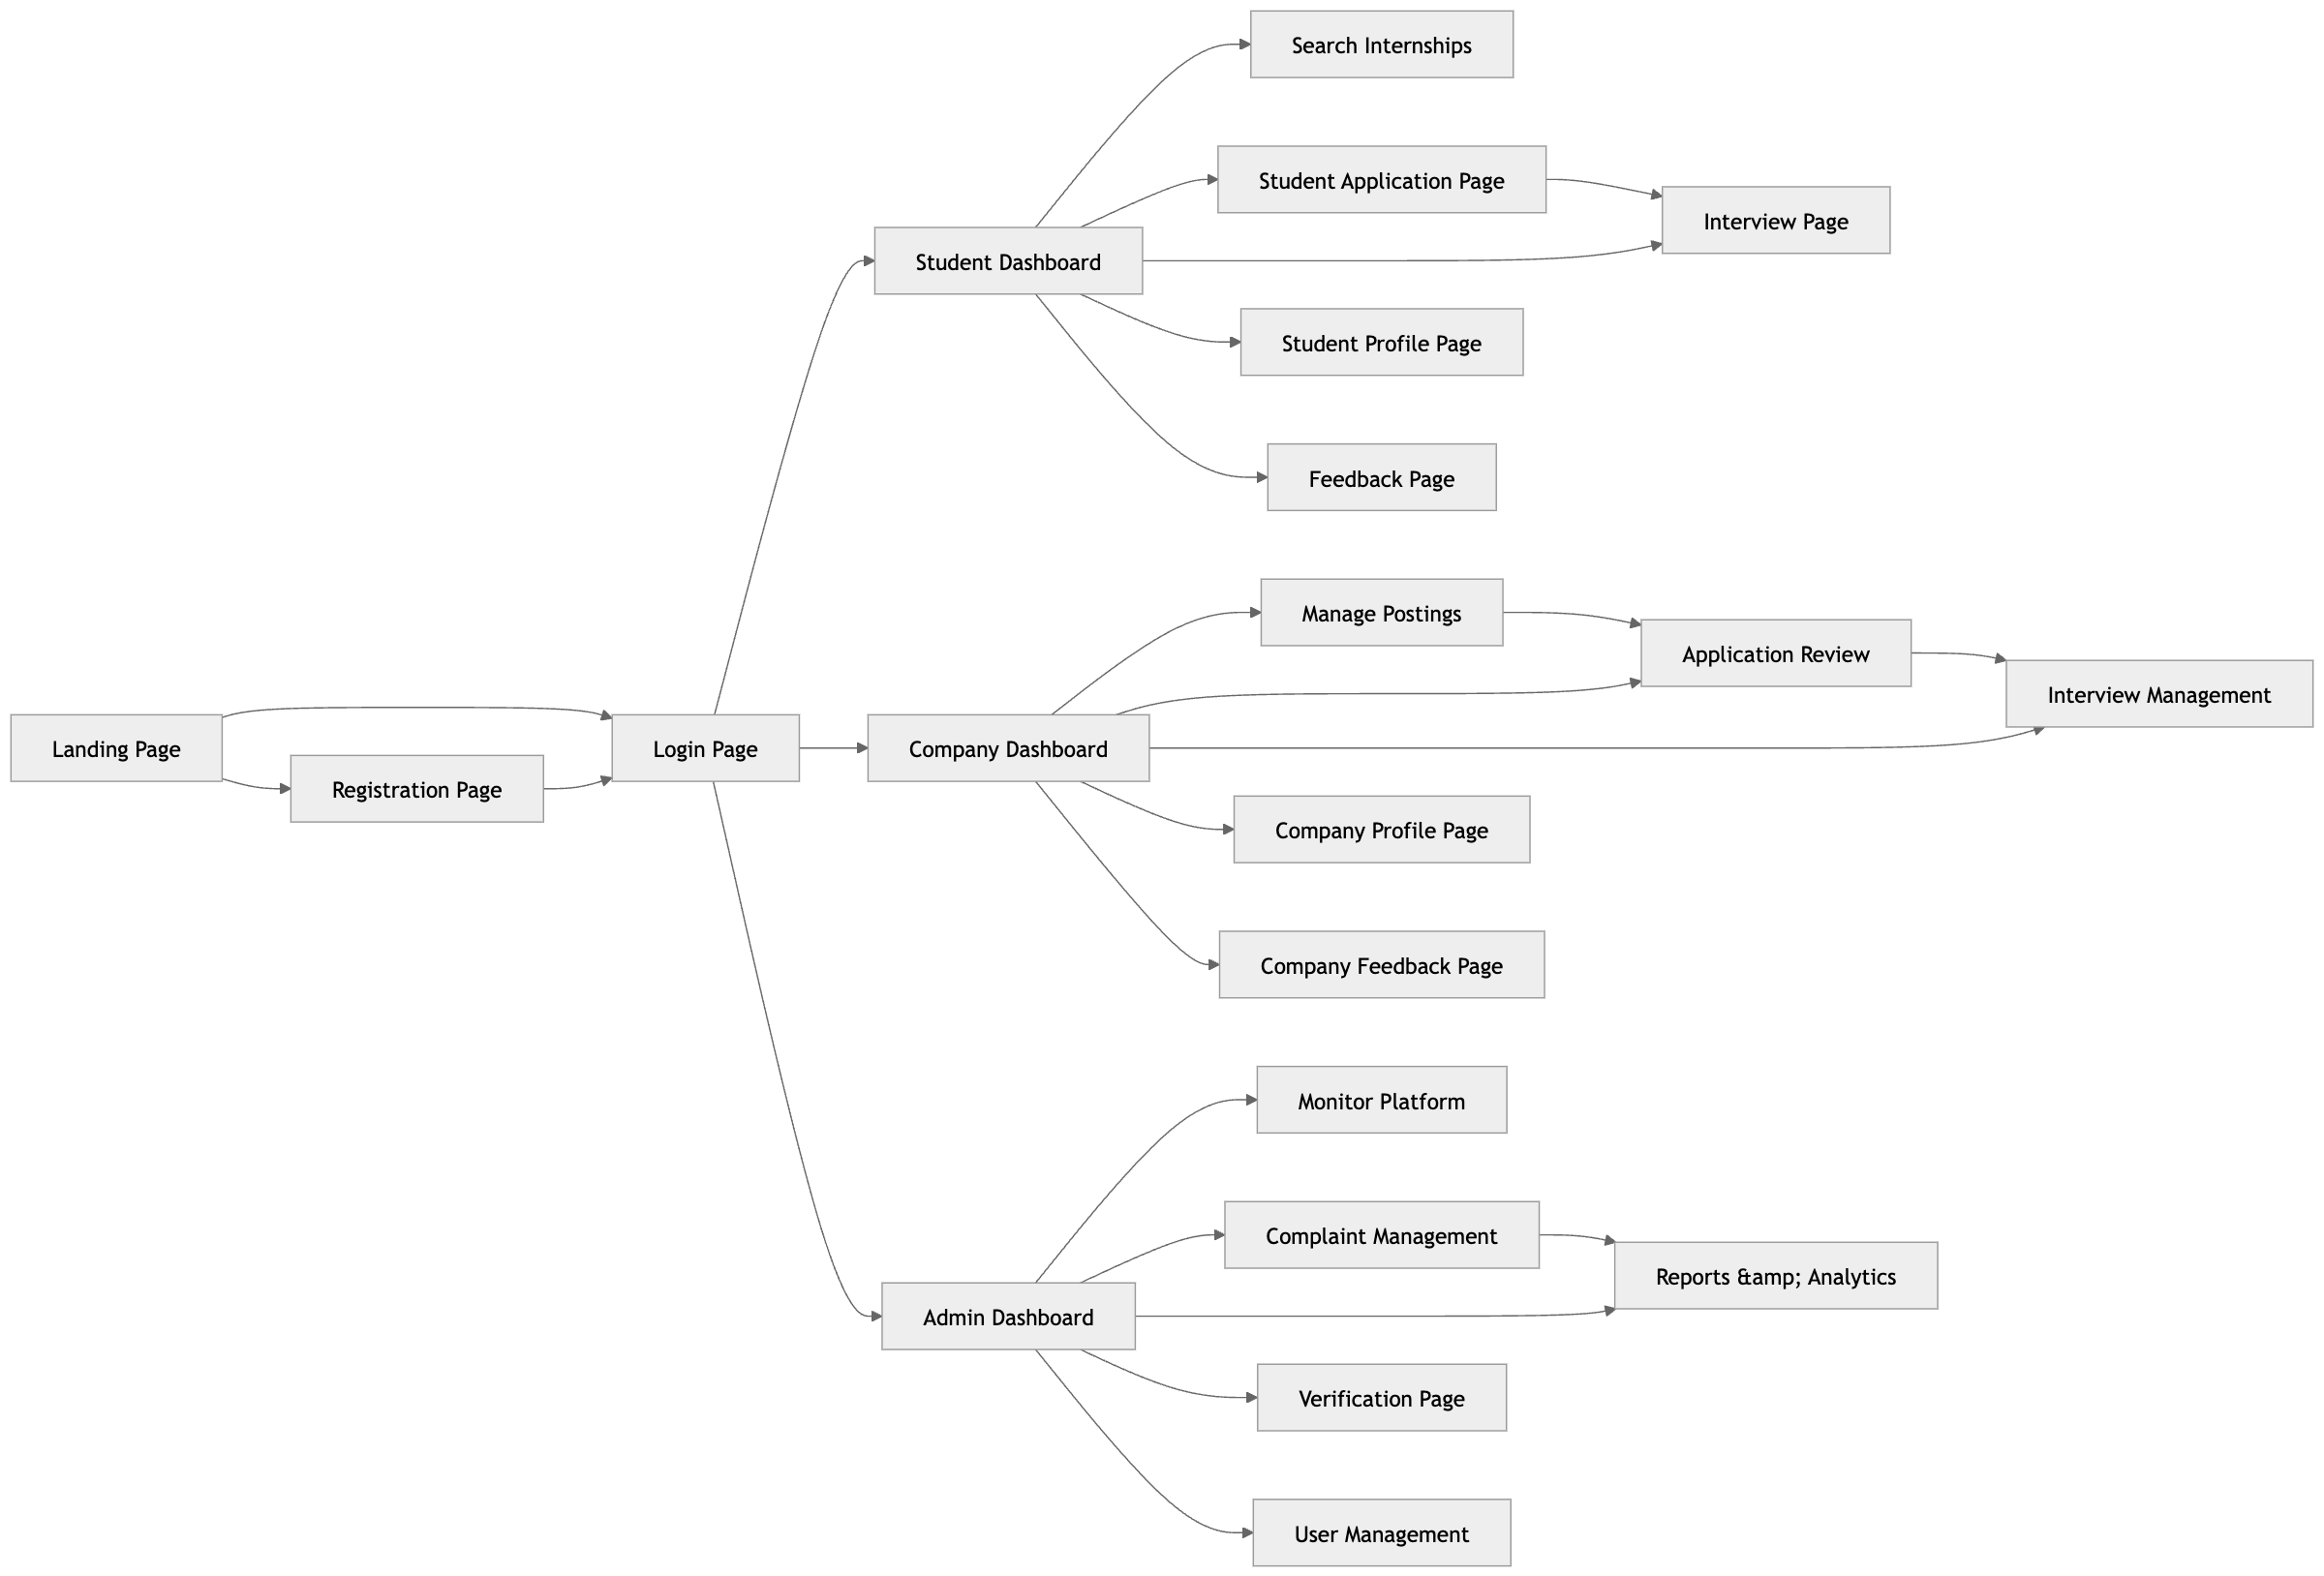
\includegraphics[width=0.82\linewidth]{JhaBhatiaSharma/imagesDD/UIOverview.png}
        \caption{UI Overview}
        \label{fig:uiOverview}
    \end{center}
\end{figure}

This graphic shows the flow and relationships between distinct pages designed for different user roles, giving a thorough overview of the \textbf{InternHub – Students \& Companies (S\&C)} platform's user interface (UI) architecture. 

\begin{enumerate}
    \item \textbf{Landing Page:} Points users to the Login Page for current users or the Registration Page for new users.
    \item \textbf{Role-Specific Dashboards:}
    \begin{itemize}
        \item \textbf{Student Dashboard:} Access to the Student Application Page, Feedback Page, Student Profile Page, Interview Management, and Search Internships.
        \item \textbf{Company Dashboard:} supports hiring processes by giving users access to the Feedback Page, Company Profile Page, and tools for managing job postings and applicant reviews.
        \item \textbf{Admin Dashboard:} Features like User Management, Complaint Management, Verification Page, and Reports \& Analytics allow for administrative monitoring.
    \end{itemize}
\end{enumerate}

This structured design emphasizes role-specific features and smooth navigation, ensuring an effective user experience for all stakeholders. The diagram's links illustrate the dynamic and scalable nature of the interface, tailored to the diverse needs of administrators, businesses, and students.

\section{User Interfaces}
\label{sec:user_interfaces}%

\subsection{UI1. Login}
\label{subsec:login_ui}%
\begin{figure}[H]
    \begin{center}
        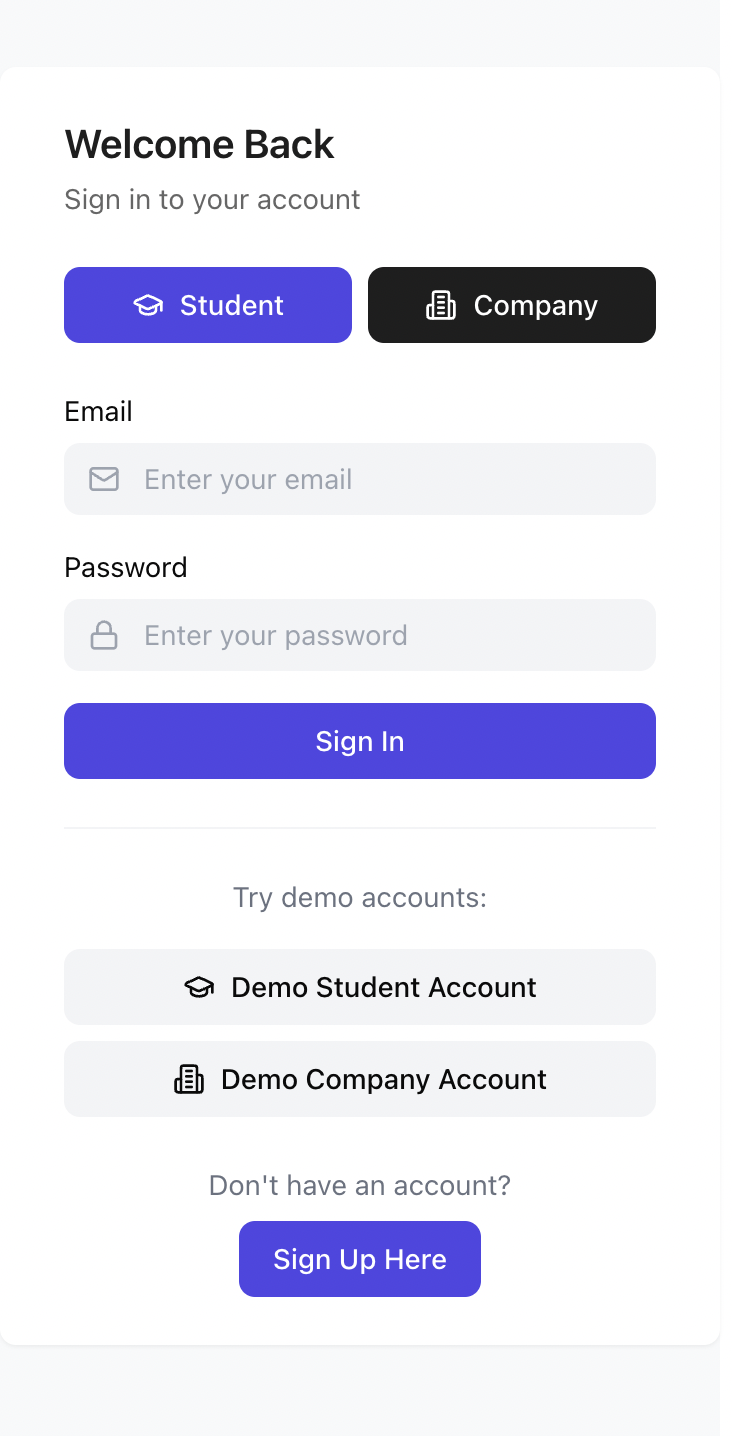
\includegraphics[width=0.52\linewidth]{JhaBhatiaSharma/imagesDD/LoginMockup.png}
        \caption{Login Interface Mockup}
        \label{fig:LoginInterface}
    \end{center}
\end{figure}
The login page is designed to provide a seamless access experience for the two main user roles: companies and students. 

\begin{enumerate}
    \item \textbf{Role Toggle:} Users can choose their role using a toggle option at the top, guaranteeing a customized login experience.
    \item \textbf{User Input Fields:} With the help of user-friendly placeholders, users enter their email address and password.
    \item \textbf{"Sign In" Button:} Prominently displayed for easy access.
    \item \textbf{Demo Accounts:} Allows users to test features without signing up.
    \item \textbf{"Sign Up Here" Link:} Redirects new users to the registration page.
\end{enumerate}

The simple, clear design ensures an intuitive experience for all users while maintaining a professional appearance.

\subsection{UI2. SignUp}
\label{subsec:signup_ui}%

\begin{figure}[H]
    \begin{center}
        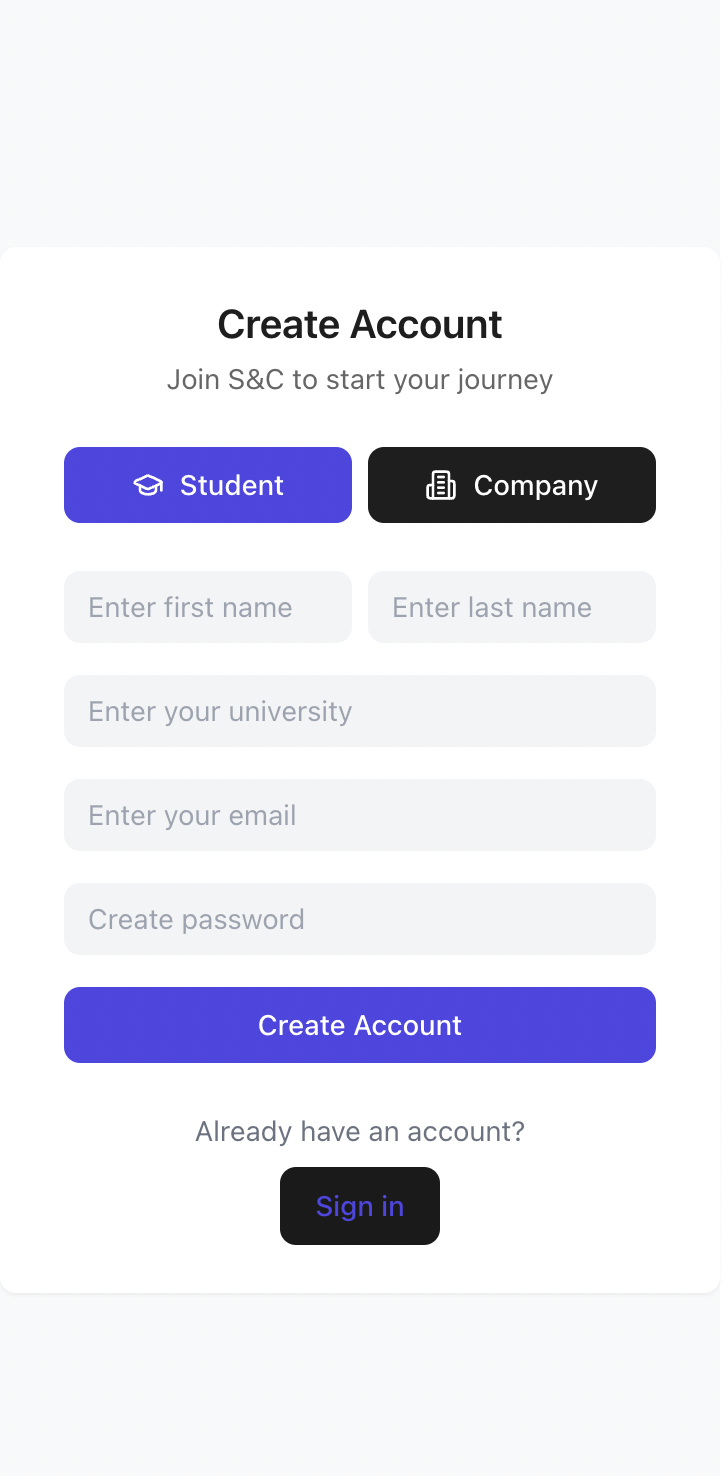
\includegraphics[width=0.52\linewidth]{JhaBhatiaSharma/imagesDD/SignUp.png}
        \caption{SignUp Interface Mockup}
        \label{fig:signupinterface}
    \end{center}
\end{figure}

The registration page provides a streamlined and user-friendly interface for new users to create accounts.

\begin{enumerate}
    \item \textbf{Role Selection:} At the top of the website, users have the option to switch between the Student and Company roles.
    \item \textbf{Input Fields:} Consists of the student's university, email, password, and first and last names.
    \item \textbf{"Create Account" Button:} Simplifies the submission process.
    \item \textbf{"Sign In" Link:} Redirects existing users to the login page.
\end{enumerate}

This design guarantees a professional and user-friendly experience for new users entering the platform.

\subsection{UI3. Company Dashboard}
\label{subsec:company_dashboard_ui}%

\begin{figure}[H]
    \begin{center}
        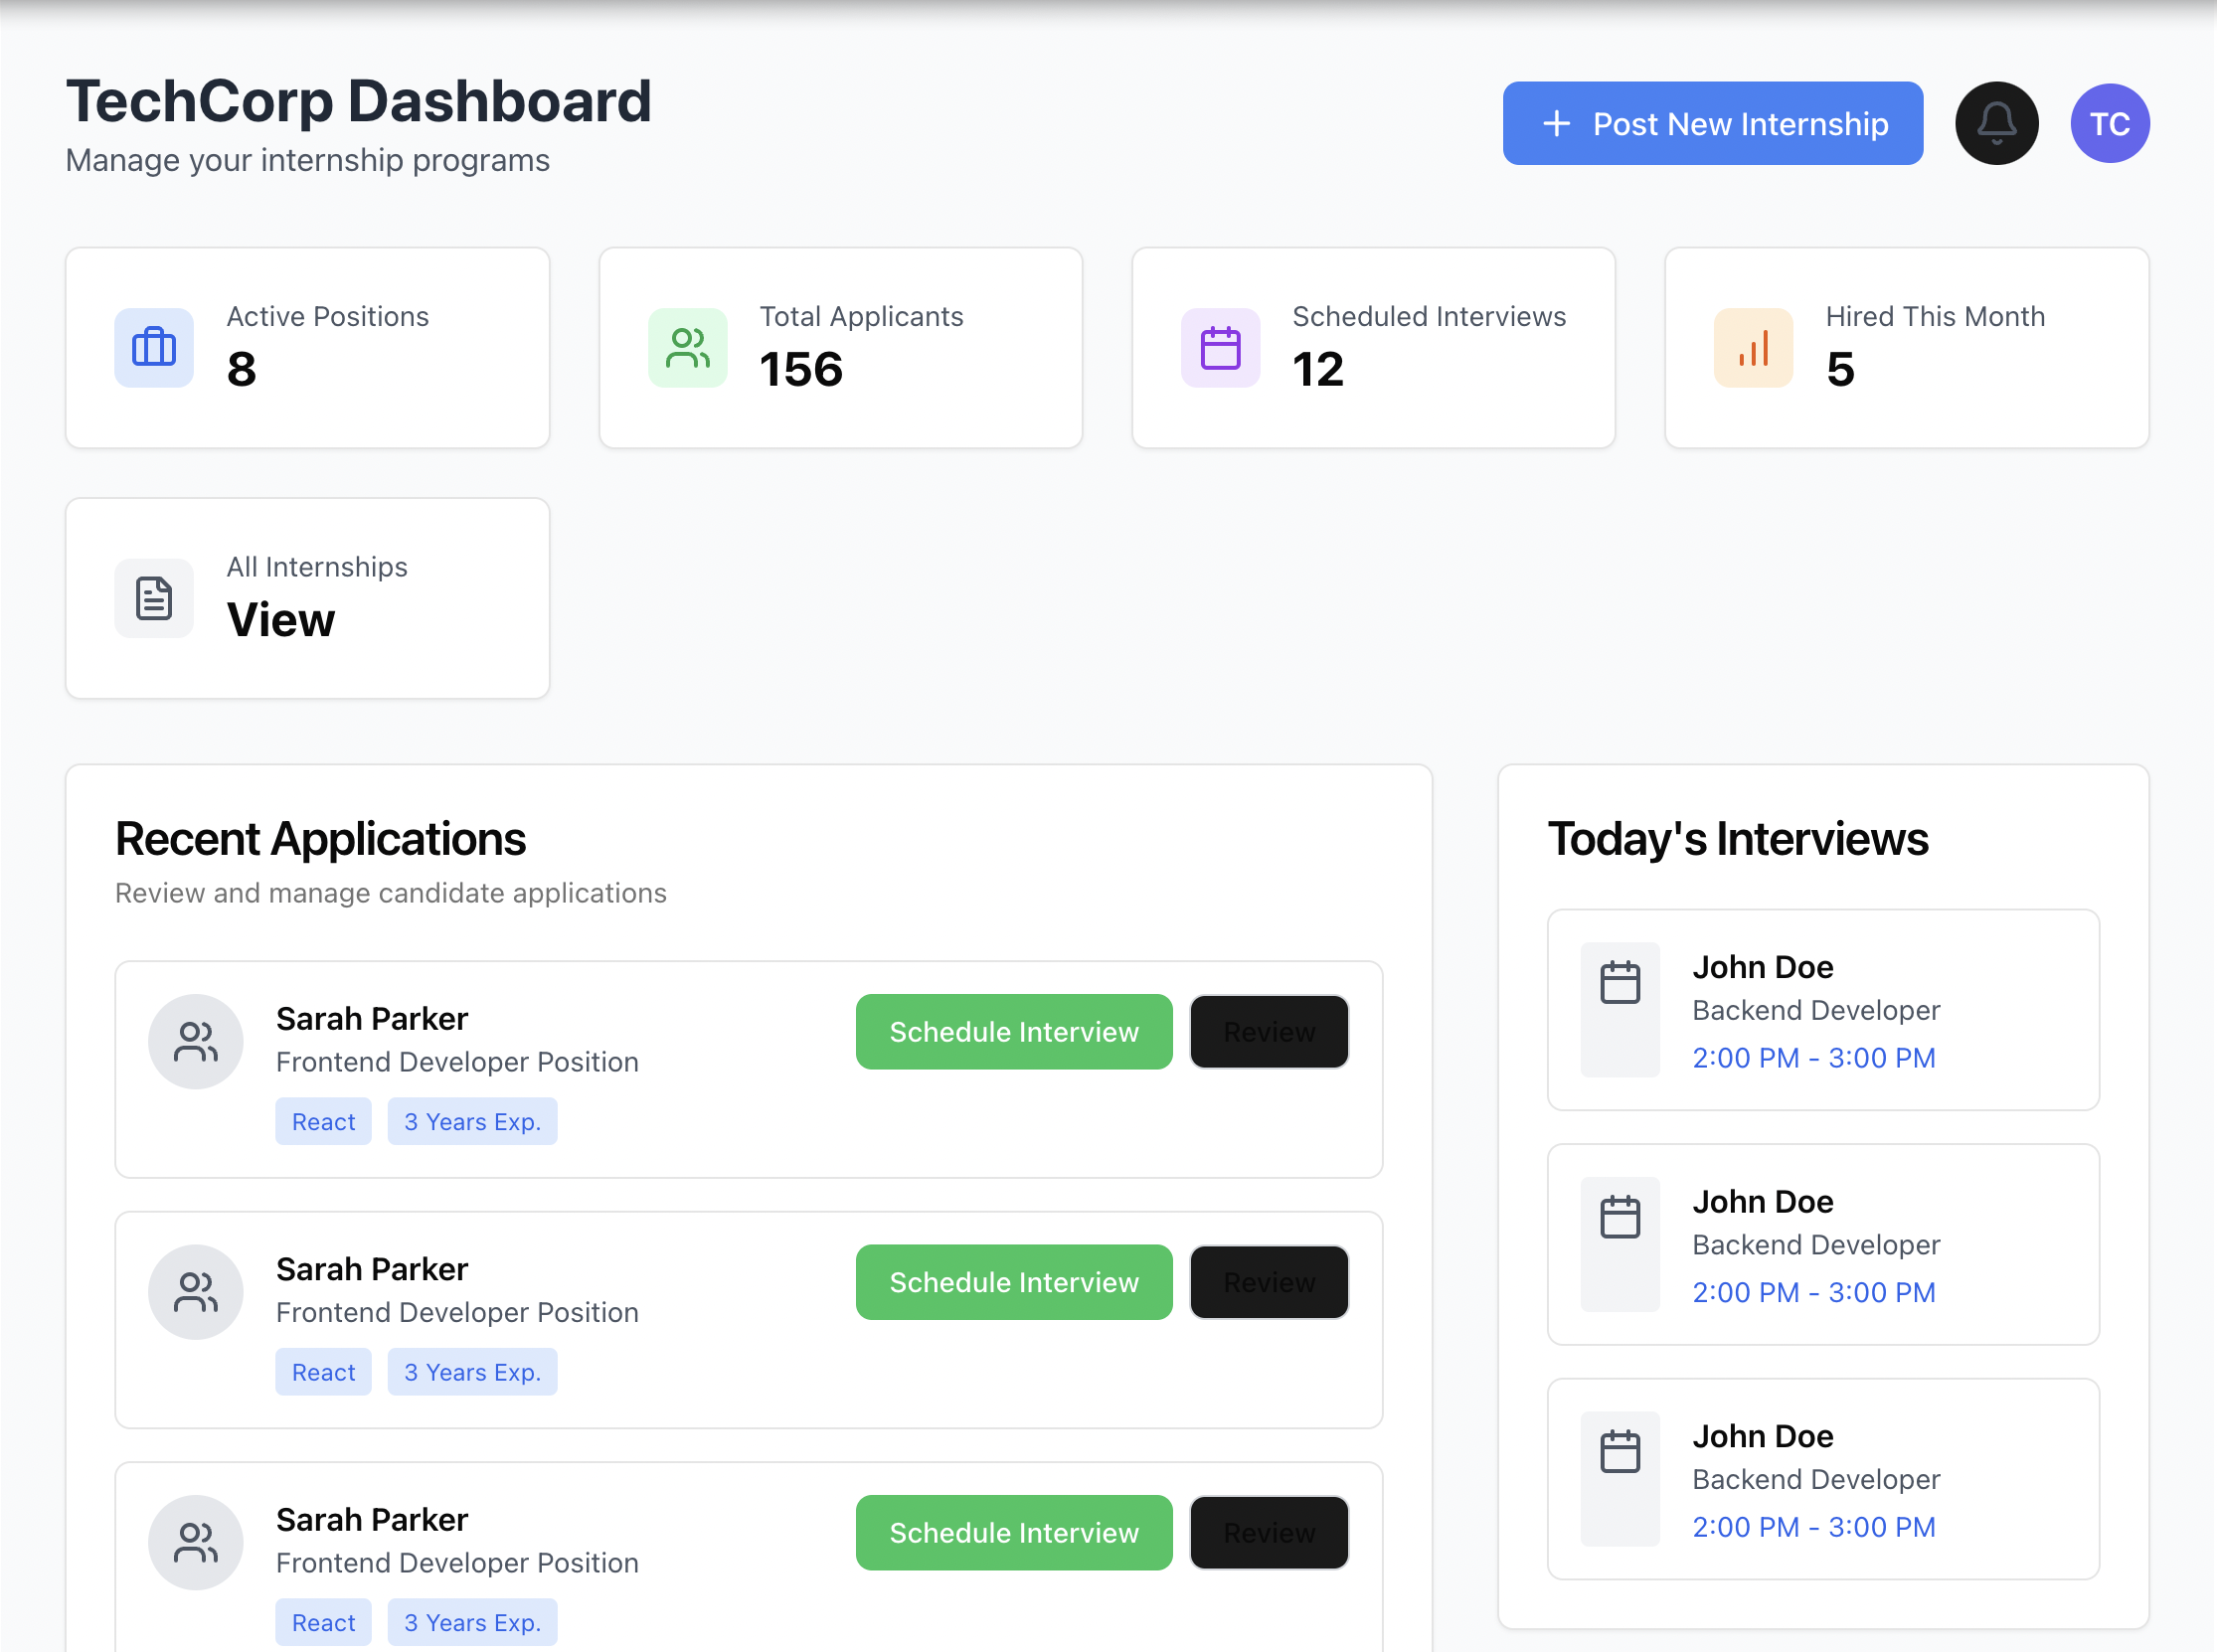
\includegraphics[width=0.82\linewidth]{JhaBhatiaSharma/imagesDD/CompanyDashboard.png}
        \caption{Company Dashboard}
        \label{fig:companyDashboard}
    \end{center}
\end{figure}

The Company Dashboard offers a well-structured interface for recruiters to efficiently manage their internship programs.

\begin{enumerate}
    \item \textbf{Dashboard Overview:} shows important information like Hired This Month, Total Applicants, Scheduled Interviews, and Active Positions.
    \item \textbf{Post Internship:} An easy-to-use button for publishing new internship opportunities.
    \item \textbf{Recent Applications:} shows applicant submissions together with pertinent information such as name, experience, talents, and position applied for. includes choices for reviewing applications or setting up interviews.
    \item \textbf{Today's Interviews:} Displays a brief interview schedule with the names, positions, and times of the candidates.
\end{enumerate}

This layout ensures all essential information is easily accessible, enabling recruiters to navigate and complete their tasks effectively.

\subsection{UI4. Post Internship}
\label{subsec:post_internship_ui}%

\begin{figure}[H]
    \begin{center}
        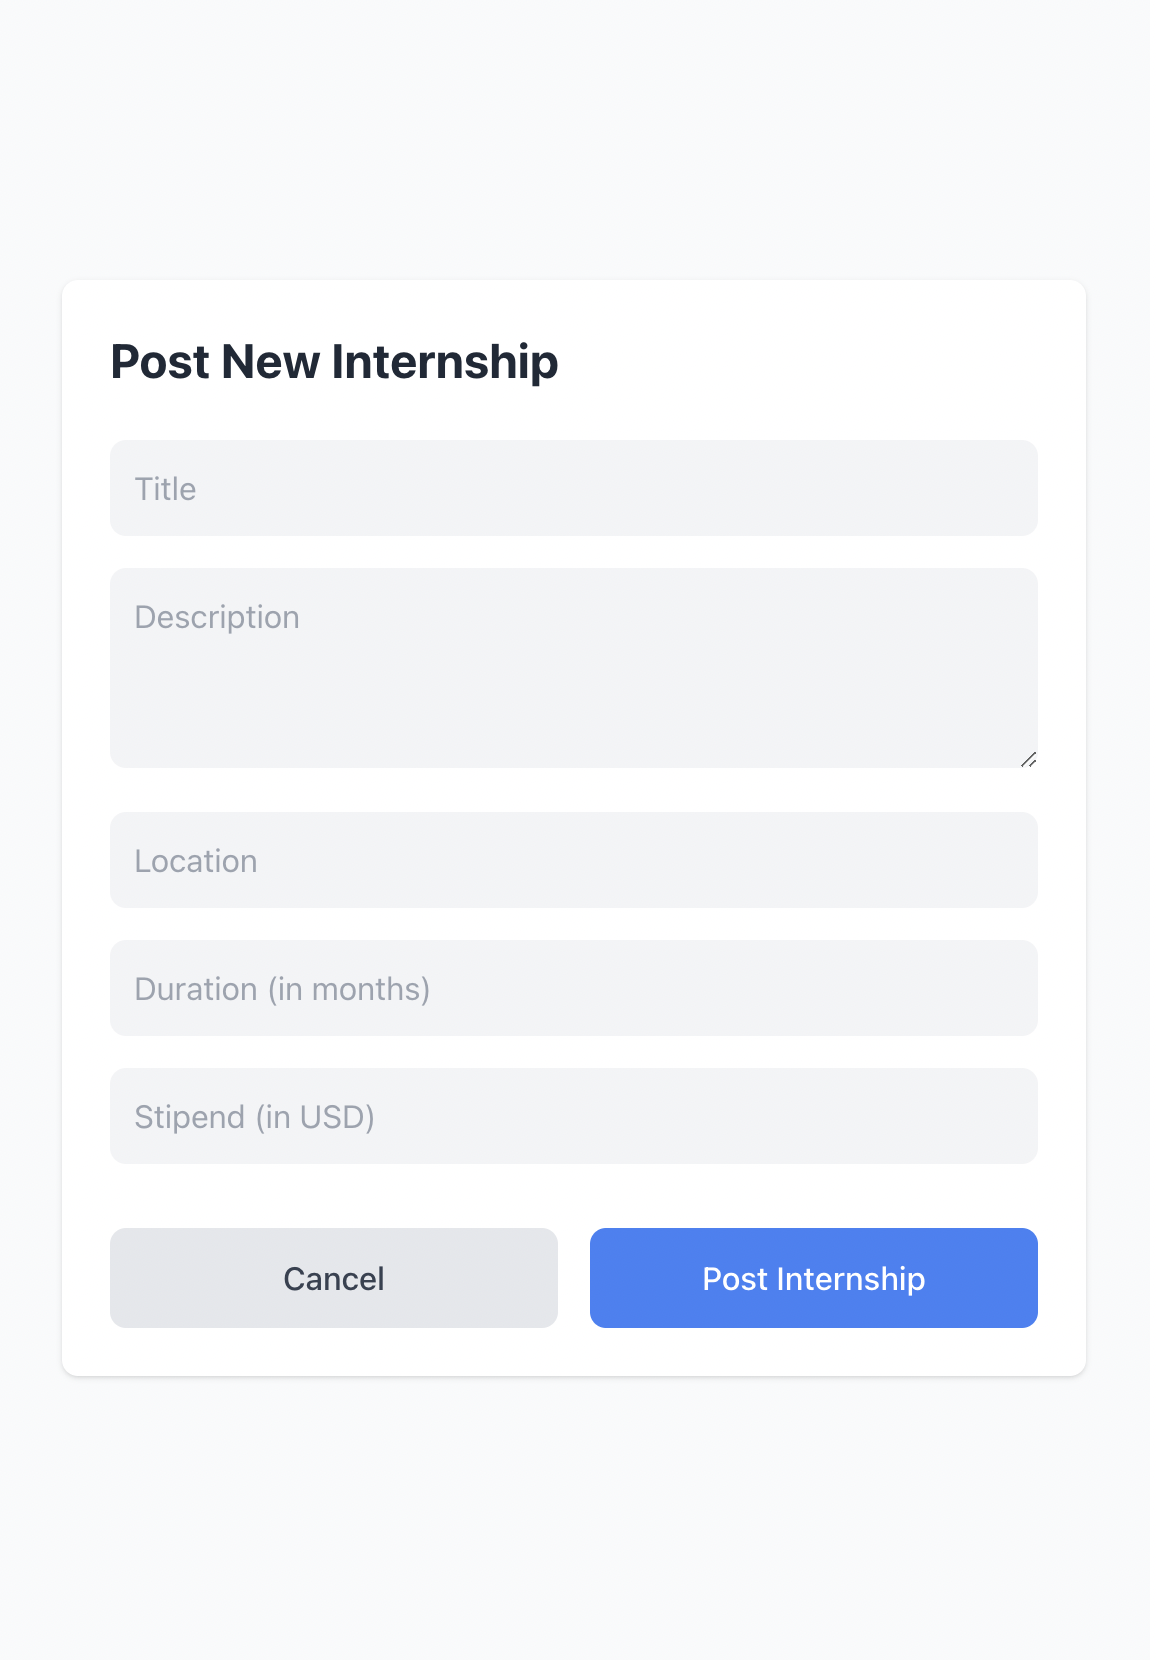
\includegraphics[width=0.62\linewidth]{JhaBhatiaSharma/imagesDD/PostInternship.png}
        \caption{Post Internship}
        \label{fig:postInternship}
    \end{center}
\end{figure}

Recruiters can post internship opportunities to the platform using a structured interface by utilizing the \textbf{Post New Internship} form. The form includes fields for essential details such as:
\begin{enumerate}
    \item \textbf{Title:} The name of the internship position.
    \item \textbf{Description:} Ccomprehensive details regarding the position and duties.
    \item \textbf{Location:} The physical or remote location of the internship.
    \item \textbf{Duration:} Length of the internship in months.
    \item \textbf{Stipend:} Details regarding the compensation offered.
\end{enumerate}

The form is designed with clearly defined and spaced fields to ensure clarity and ease of use. At the bottom, a \textbf{Post Internship} button enables submission of the internship details, while a \textbf{Cancel} button allows recruiters to terminate the process. This arrangement prioritizes simplicity and functionality, enabling businesses to efficiently communicate openings to prospective candidates.

\subsection{UI5. Student Dashboard}
\label{subsec:student_dashboard_ui}%
\begin{figure}[H]
    \begin{center}
        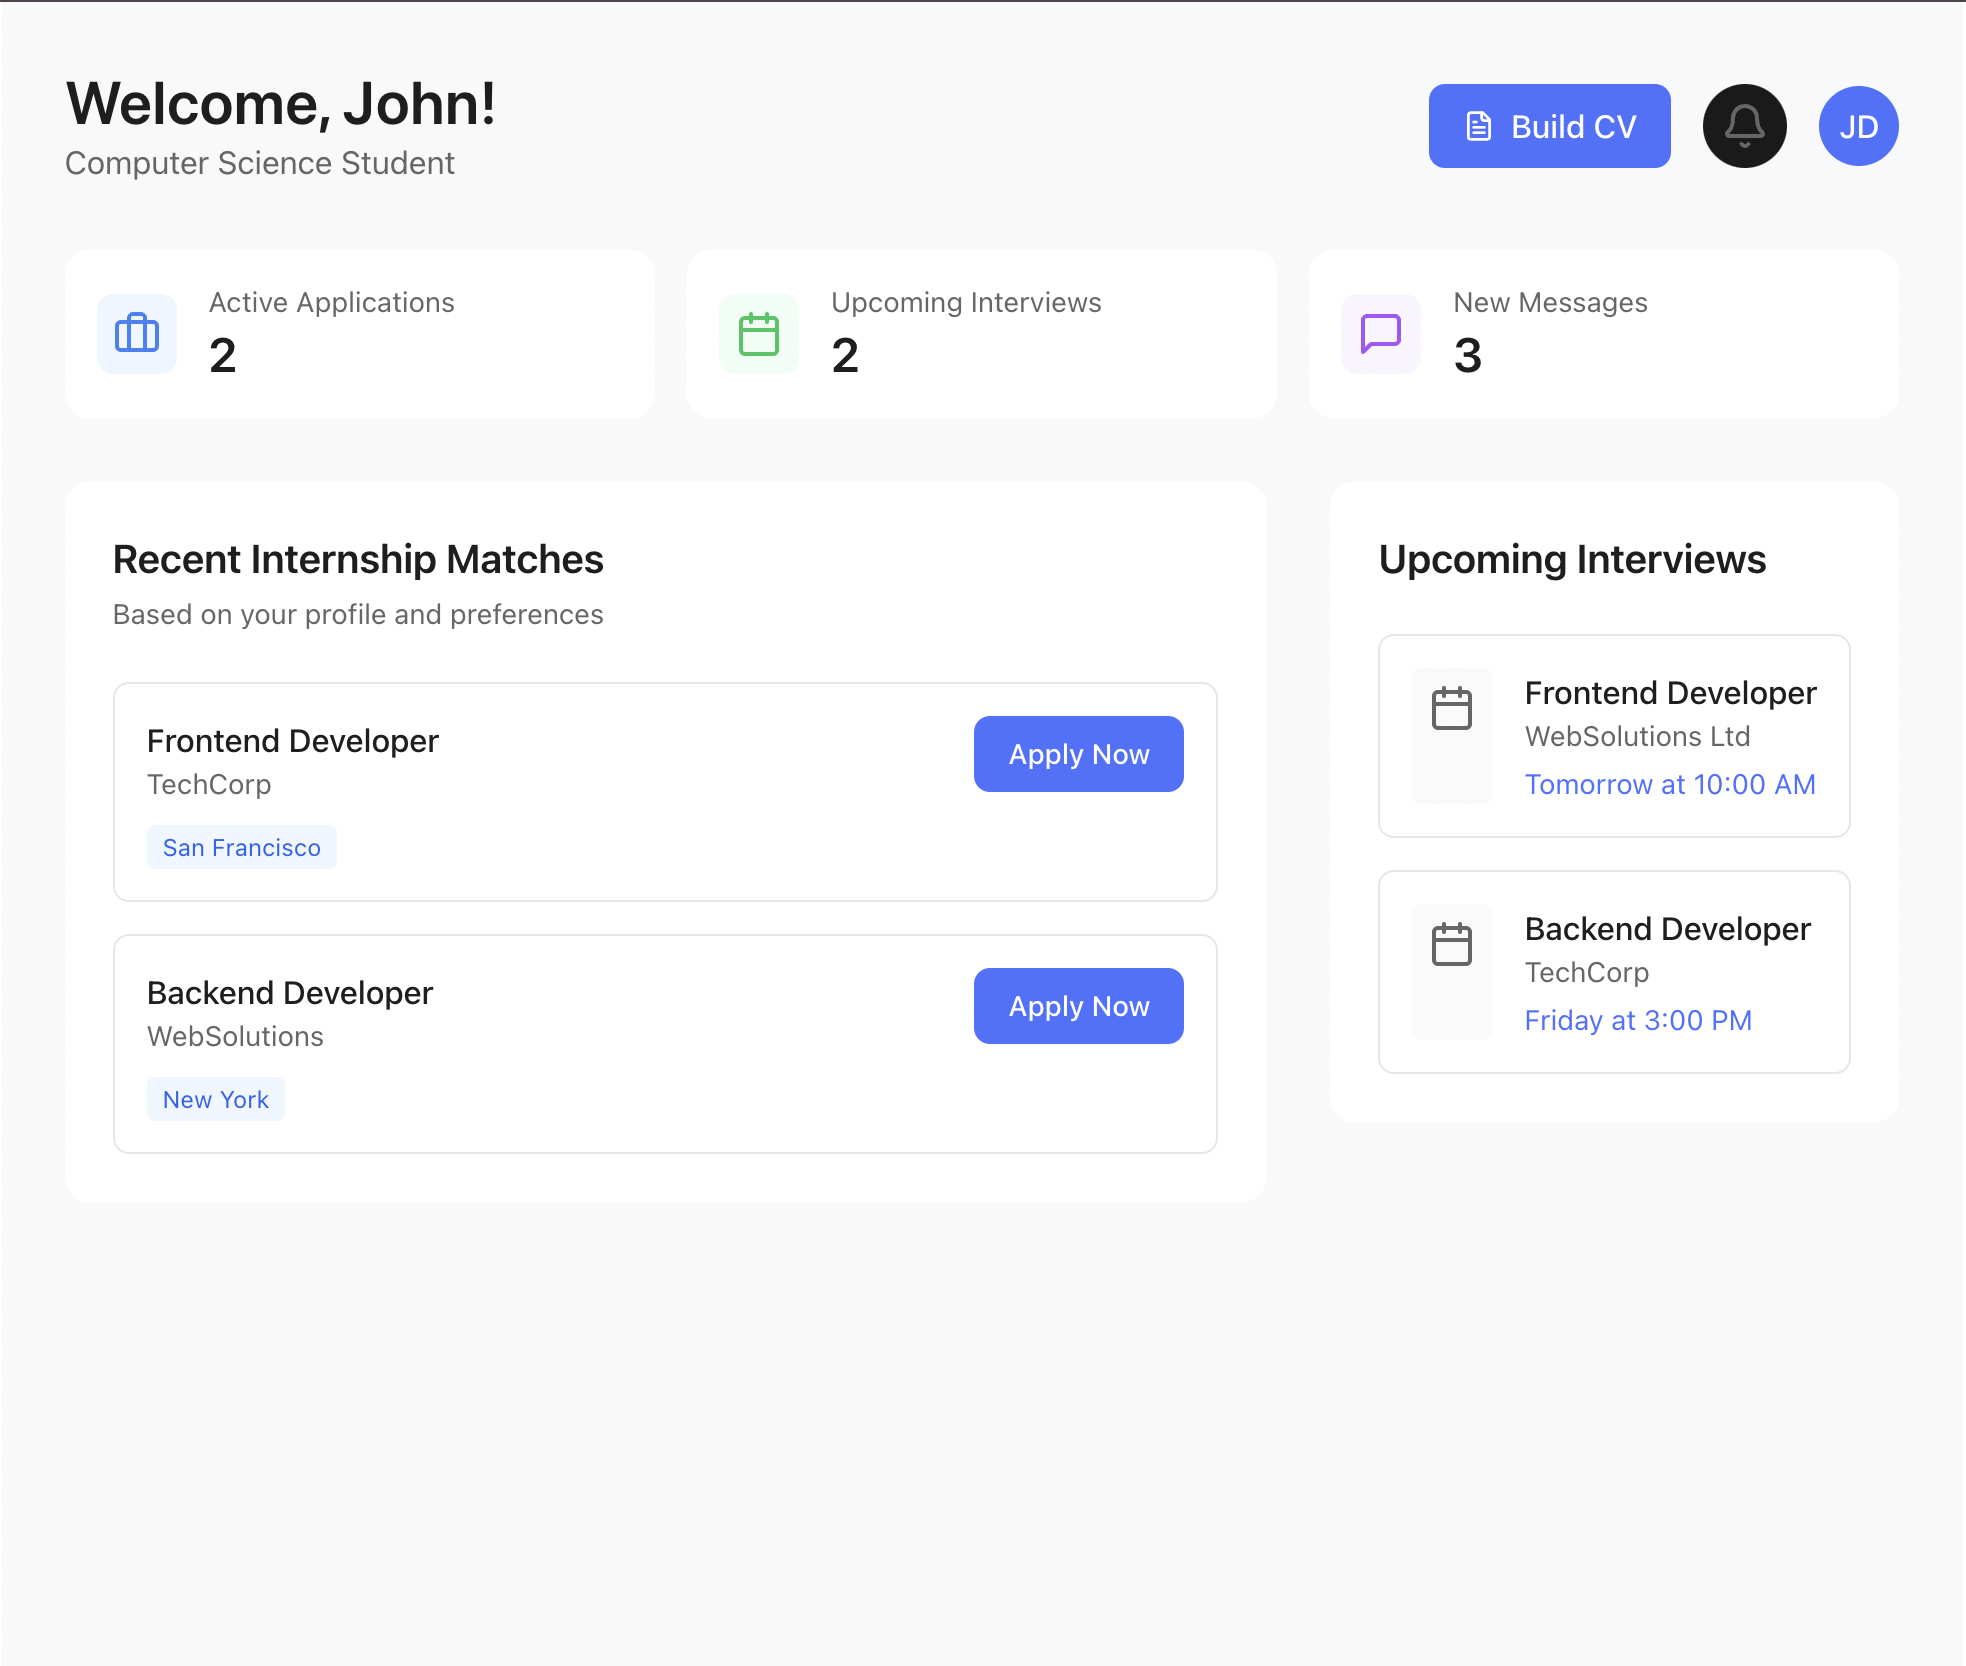
\includegraphics[width=0.82\linewidth]{JhaBhatiaSharma/imagesDD/StudentDashboard.png}
        \caption{Student Dashboard}
        \label{fig:studentDashboard}
    \end{center}
\end{figure}

The \textbf{Student Dashboard} provides a customized and streamlined interface to help students effectively manage their internship applications and search processes. Key features include:
\begin{enumerate}
    \item \textbf{Overview:} Shows important indicators like New Messages, Upcoming Interviews, and Active Applications.
    \item \textbf{Build CV:} A button to access resume-building resources.
    \item \textbf{Recent Internship Matches:} Shows internship opportunities tailored to the student's profile and preferences, including roles like Frontend Developer and Backend Developer, with company names, locations, and an \textbf{Apply Now} button for quick action.
    \item \textbf{Upcoming Interviews:} Shows the time, employer, and position details for the planned interviews.
\end{enumerate}

The layout emphasizes accessibility and relevance, ensuring students can quickly find and act on the most important information to enhance their internship experience.

\subsection{UI6. Build CV}
\label{subsec:build_cv_ui}%

\begin{figure}[H]
    \begin{center}
        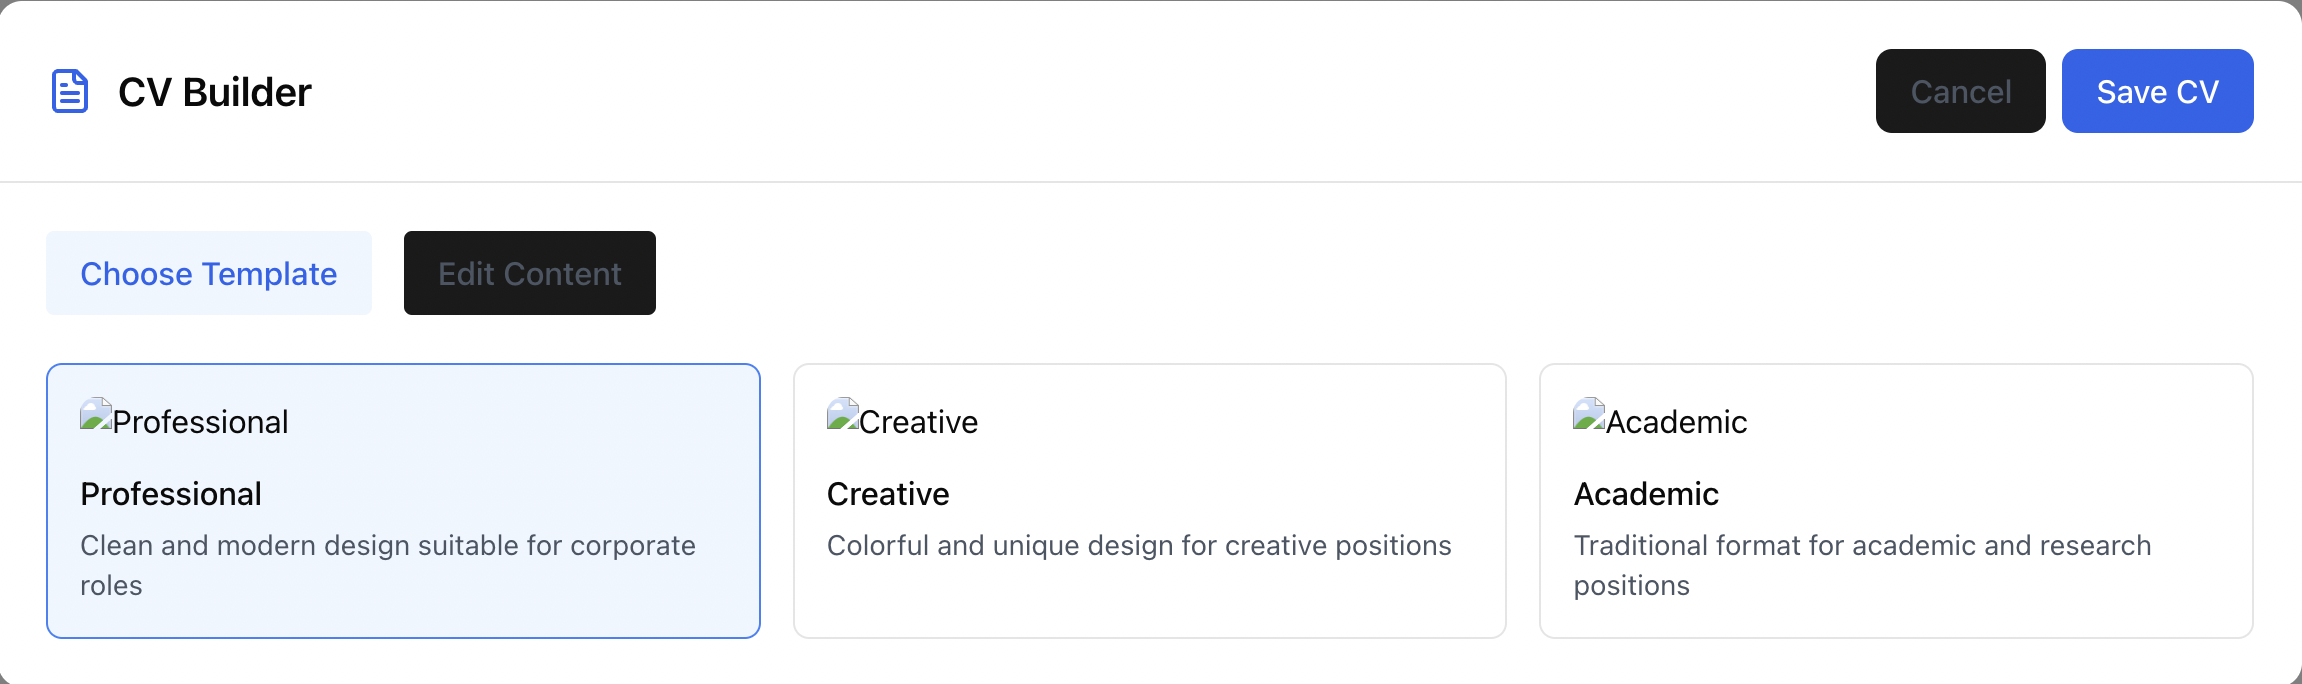
\includegraphics[width=0.82\linewidth]{JhaBhatiaSharma/imagesDD/BuildCV.png}
        \caption{Build CV}
        \label{fig:BuildCV}
    \end{center}
\end{figure}

The \textbf{CV Builder} interface provides a simplified and well-structured layout that enables users to create and modify resumes. The interface includes two primary steps:
\begin{enumerate}
    \item \textbf{Choose Template:}To help users choose the ideal format for their career goals and the kind of position they are aiming for, users can choose from three options: Professional, Creative, and Academic. Each choice has an explanation.
    \item \textbf{Edit Content:} Users can personalize their resumes by adding their education, employment experience, talents, and personal details.
\end{enumerate}

Users can \textbf{Cancel} changes or \textbf{Save CV} to finalize their resume using buttons in the upper-right corner. This design ensures users can efficiently create resumes tailored to their professional needs while maintaining simplicity and clarity throughout the process.

\subsection{UI7. Messaging System}
\label{subsec:messaging_system_ui}%

\begin{figure}[H]
    \begin{center}
        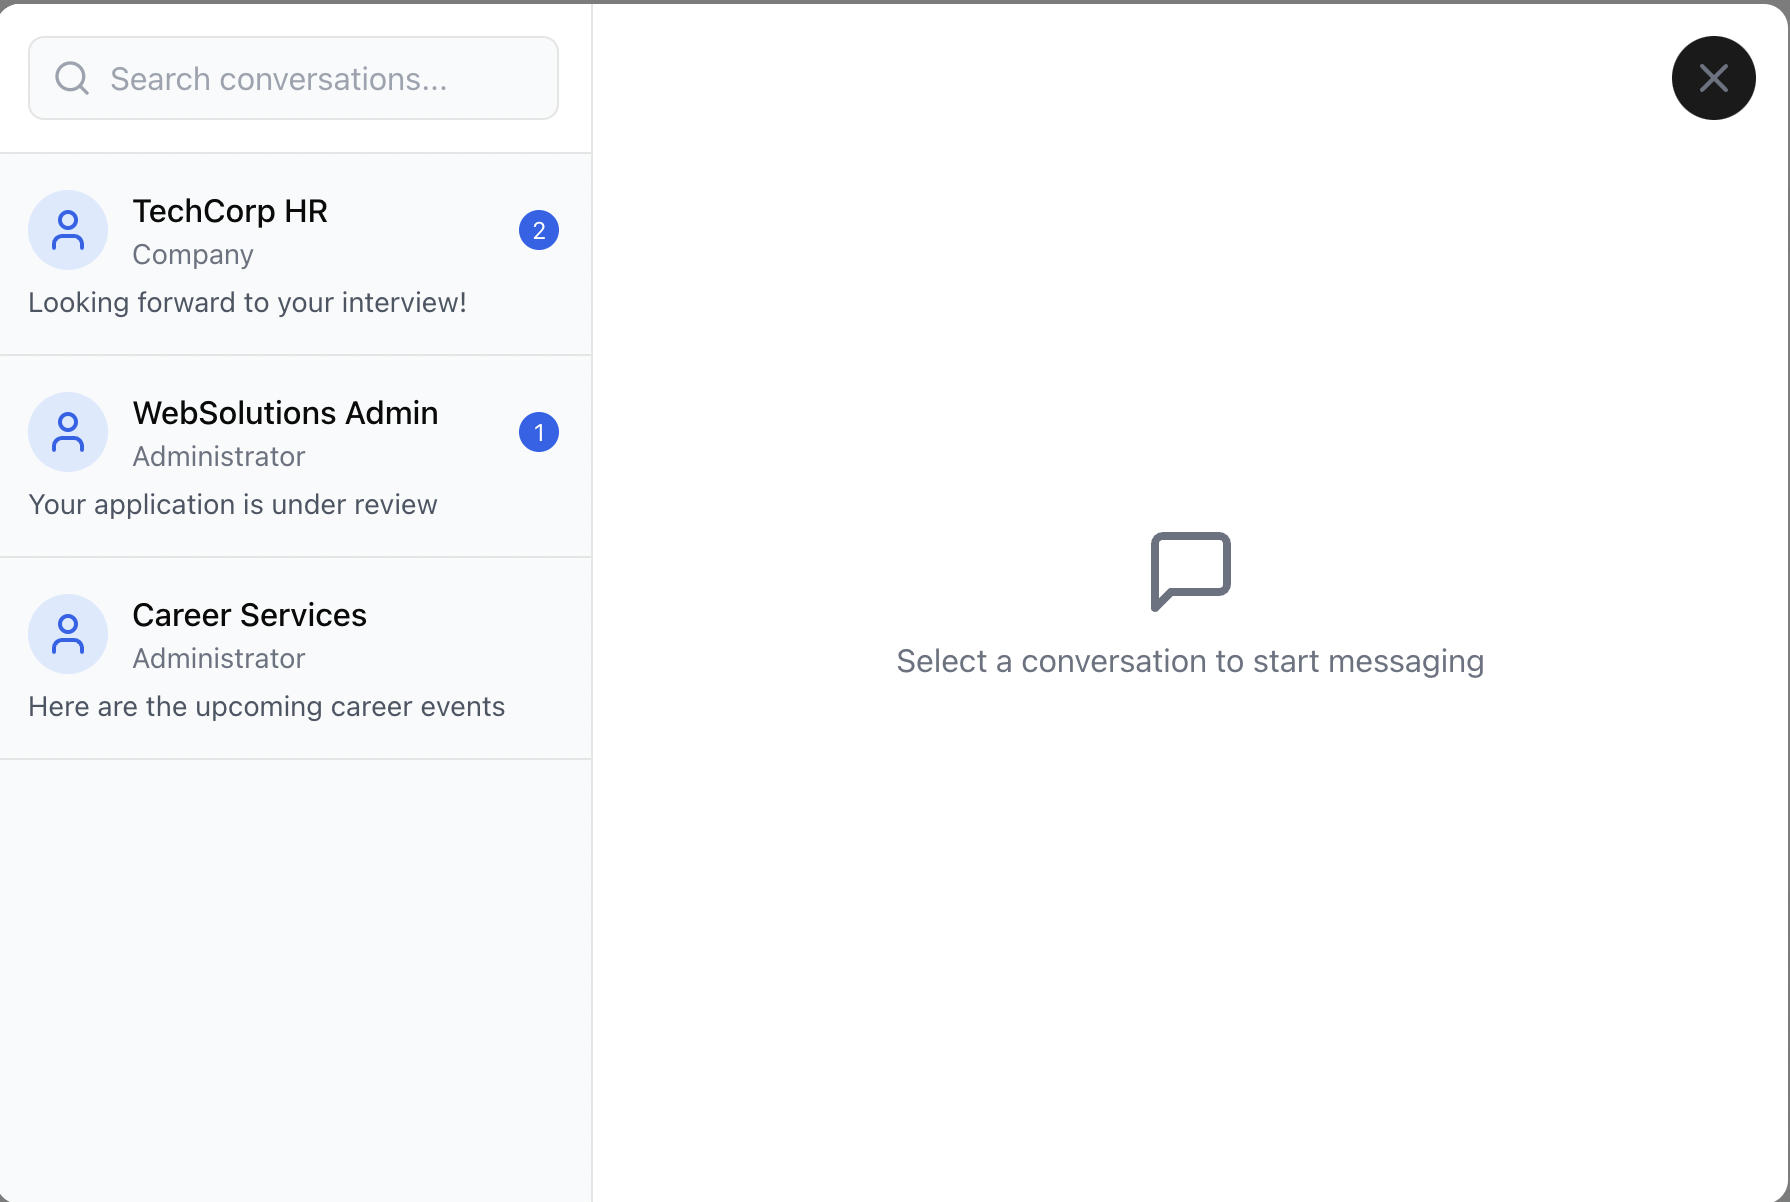
\includegraphics[width=0.70\linewidth]{JhaBhatiaSharma/imagesDD/MessagingSystem.png}
        \caption{Messaging System}
        \label{fig:messagingSystme}
    \end{center}
\end{figure}

The \textbf{Messaging System} interface enables users to have seamless conversations with various stakeholders on the \textbf{InternHub – Students \& Companies (S\&C)} platform. Key features include:
\begin{enumerate}
    \item \textbf{Conversation List:} Arranged on the left, displaying ongoing conversations together with information such as the contact's name, role (e.g., Administrator, Company), and a synopsis of the most recent message. The quantity of unread messages is indicated by blue badges.
    \item \textbf{Chat Panel:} The chosen chat is shown in the right panel. Here, users can send and view messages. A placeholder asks the user to select a discussion if none is selected.
    \item \textbf{Search Bar:} Located at the top of the conversation list, it allows users to look for particular conversations.
\end{enumerate}

This split-pane design ensures users can easily navigate their conversations and focus on ongoing chats without interruptions. The interface supports real-time updates, facilitating efficient communication and collaboration between administrators, businesses, and students.

